% Editable native annotations around unchanged verified IDE photographs.
\par
\begin{figure}[htbp]
\centering
\newsavebox{\MARSwavboundaryregistersBox}
\sbox{\MARSwavboundaryregistersBox}{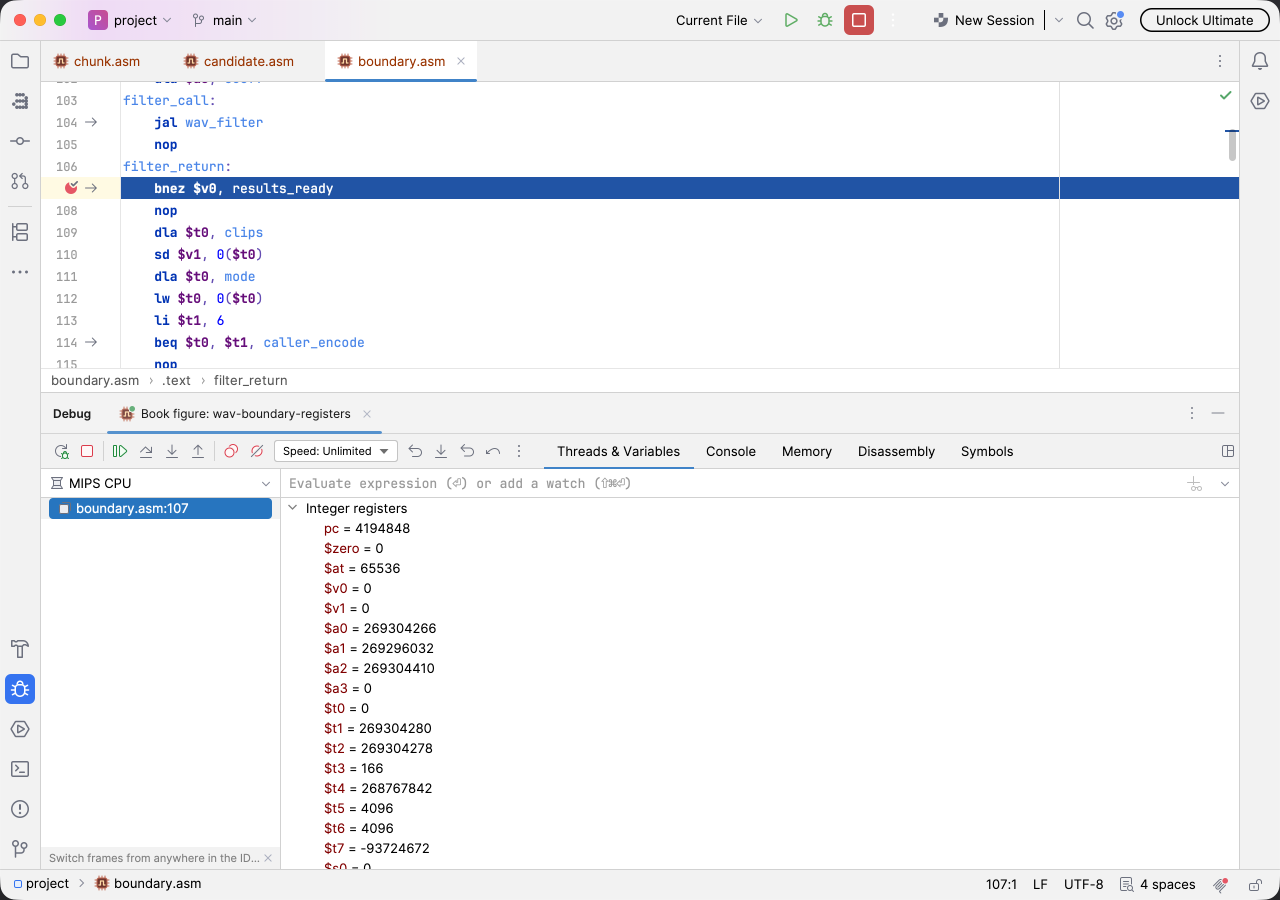
\includegraphics[artifact]{packages/031-pcm-wav/captures/f04/registers.png}}
\newsavebox{\MARSwavboundarysamplesBox}
\sbox{\MARSwavboundarysamplesBox}{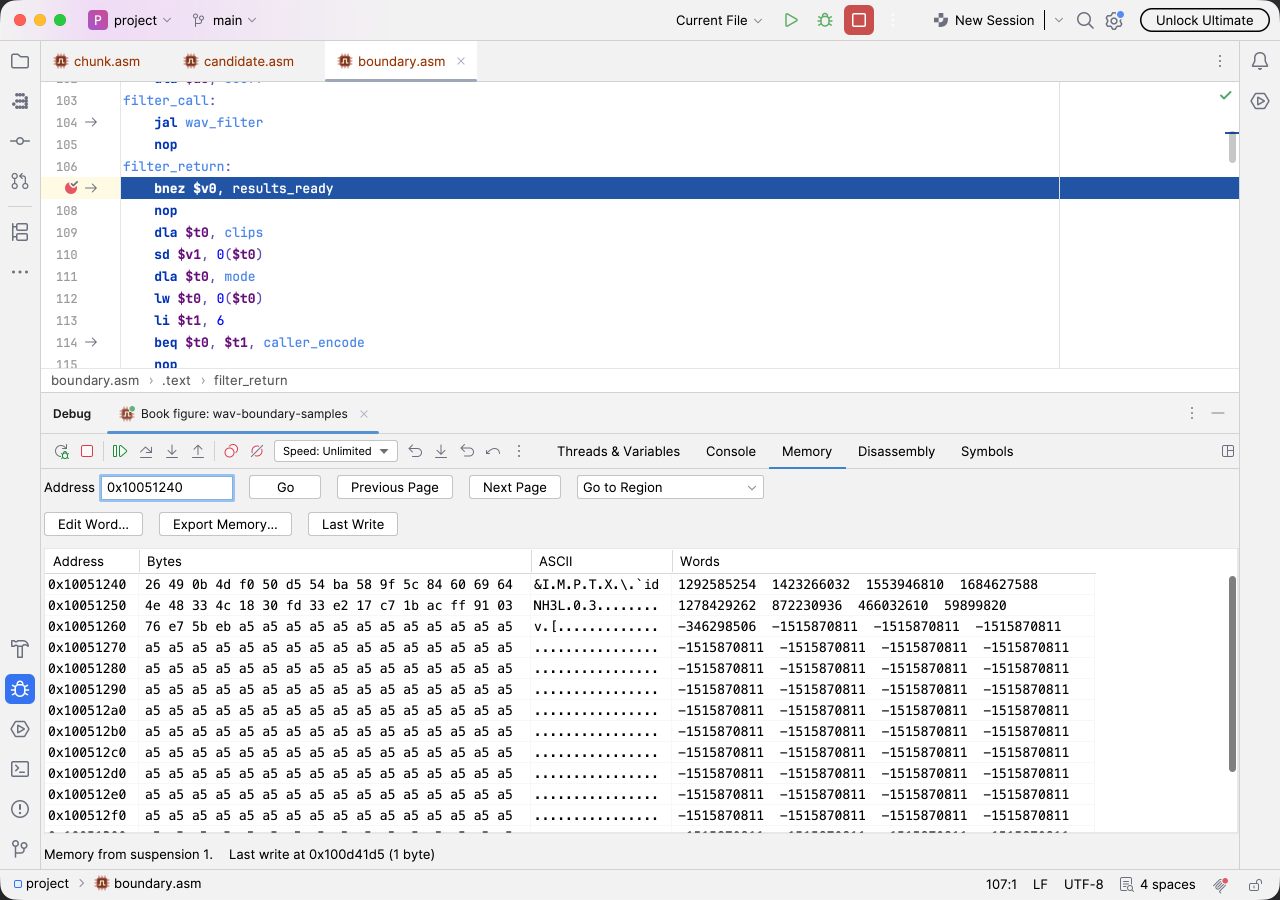
\includegraphics[artifact]{packages/031-pcm-wav/captures/f04/samples.png}}
\edef\MARSwavboundarysourceLeft{\the\dimexpr0.036718750\wd\MARSwavboundaryregistersBox\relax}
\edef\MARSwavboundarysourceBottom{\the\dimexpr0.774444444\ht\MARSwavboundaryregistersBox\relax}
\edef\MARSwavboundarysourceRight{\the\dimexpr0.713281250\wd\MARSwavboundaryregistersBox\relax}
\edef\MARSwavboundarysourceTop{\the\dimexpr0.170000000\ht\MARSwavboundaryregistersBox\relax}
\edef\MARSwavboundaryreturnsLeft{\the\dimexpr0.246093750\wd\MARSwavboundaryregistersBox\relax}
\edef\MARSwavboundaryreturnsBottom{\the\dimexpr0.312222222\ht\MARSwavboundaryregistersBox\relax}
\edef\MARSwavboundaryreturnsRight{\the\dimexpr0.553906250\wd\MARSwavboundaryregistersBox\relax}
\edef\MARSwavboundaryreturnsTop{\the\dimexpr0.640000000\ht\MARSwavboundaryregistersBox\relax}
\edef\MARSwavboundaryoutputLeft{\the\dimexpr0.034375000\wd\MARSwavboundarysamplesBox\relax}
\edef\MARSwavboundaryoutputBottom{\the\dimexpr0.287777778\ht\MARSwavboundarysamplesBox\relax}
\edef\MARSwavboundaryoutputRight{\the\dimexpr0.584375000\wd\MARSwavboundarysamplesBox\relax}
\edef\MARSwavboundaryoutputTop{\the\dimexpr0.608888889\ht\MARSwavboundarysamplesBox\relax}
\begin{tikzpicture}[alt={Three details at filter_return show the caller instruction, successful status and zero clips, and stereo output frames 56 through 64 followed by untouched sentinel bytes.}]
\node[anchor=north west,inner sep=0,font=\small\bfseries] (source-title) at (6mm,0) {Caller instruction after filtering};
\node[anchor=north west,inner sep=0] (source) at ([yshift=-1mm]source-title.south west) {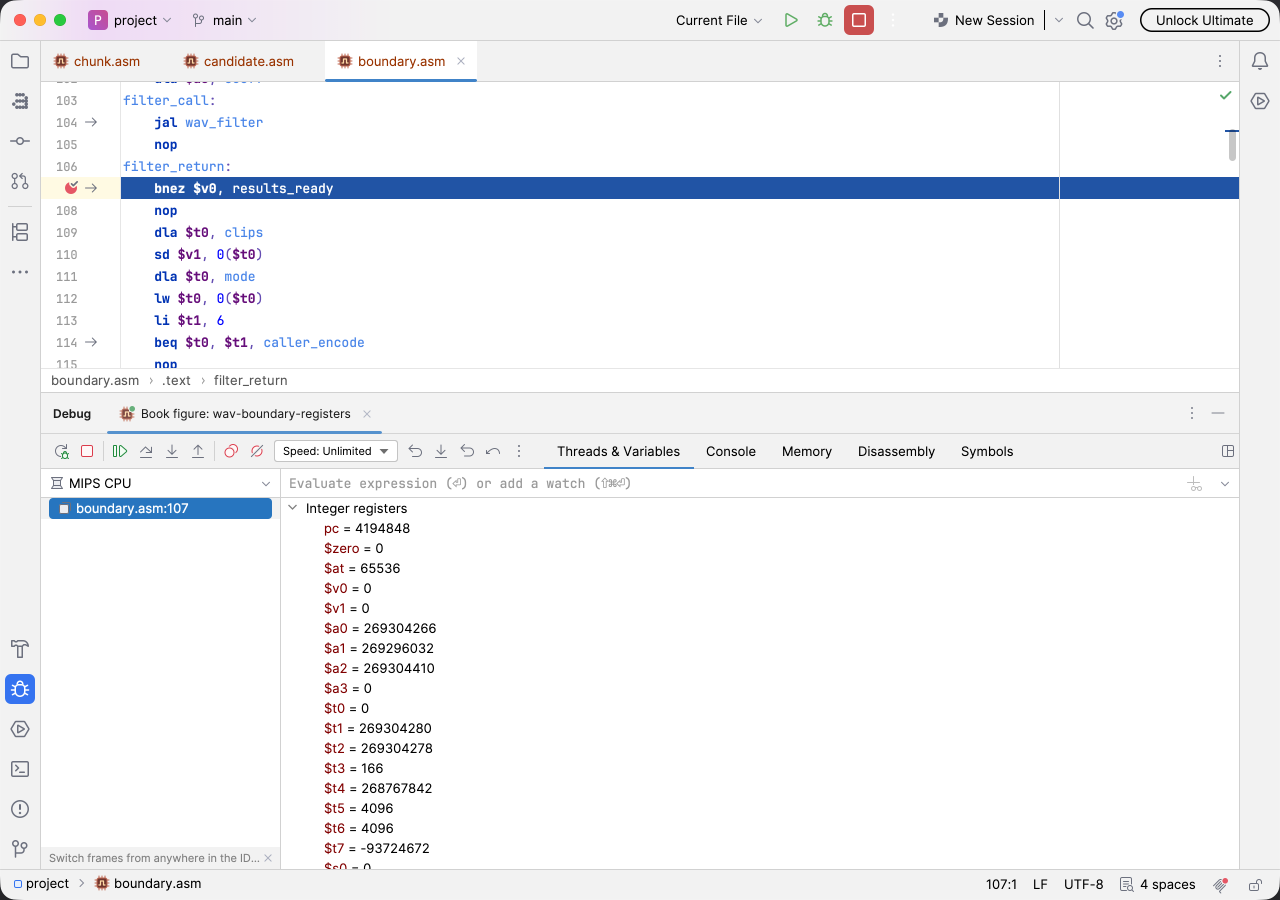
\includegraphics[width=0.54\linewidth,artifact,trim={\MARSwavboundarysourceLeft{} \MARSwavboundarysourceBottom{} \MARSwavboundarysourceRight{} \MARSwavboundarysourceTop{}},clip]{packages/031-pcm-wav/captures/f04/registers.png}};
\begin{scope}[shift={(source.south west)},x={($(source.south east)-(source.south west)$)},y={($(source.north west)-(source.south west)$)}]
\draw[black,line width=0.7pt] (0.237500000,0.080000000) rectangle (0.893750000,0.520000000);
\node[draw=black,fill=white,circle,inner sep=1.5pt,font=\footnotesize] at ($(0.237500000,0.520000000)+(-3mm,0)$) {1};
\end{scope}
\node[anchor=north west,inner sep=0,font=\small\bfseries] (returns-title) at ([yshift=-1mm]source.south west) {Success and clipped-sample count};
\node[anchor=north west,inner sep=0] (returns) at ([yshift=-1mm]returns-title.south west) {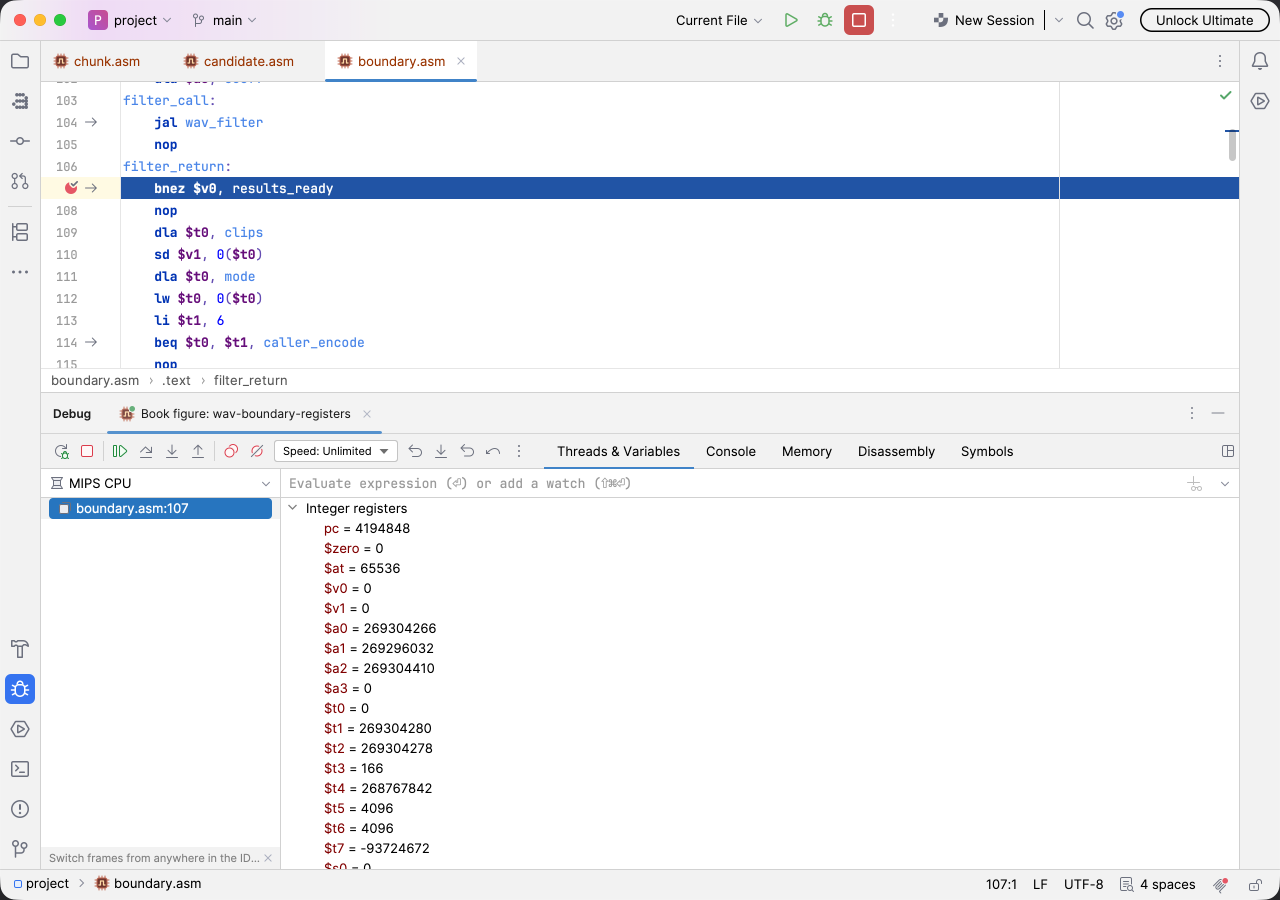
\includegraphics[width=0.44\linewidth,artifact,trim={\MARSwavboundaryreturnsLeft{} \MARSwavboundaryreturnsBottom{} \MARSwavboundaryreturnsRight{} \MARSwavboundaryreturnsTop{}},clip]{packages/031-pcm-wav/captures/f04/registers.png}};
\begin{scope}[shift={(returns.south west)},x={($(returns.south east)-(returns.south west)$)},y={($(returns.north west)-(returns.south west)$)}]
\draw[black,line width=0.7pt] (0.023437500,0.023255814) rectangle (0.226562500,0.953488372);
\node[draw=black,fill=white,circle,inner sep=1.5pt,font=\footnotesize] at ($(0.023437500,0.953488372)+(-3mm,0)$) {2};
\end{scope}
\node[anchor=north west,inner sep=0,font=\small\bfseries] (output-title) at ([yshift=-1mm]returns.south west) {Final nine stereo frames and untouched suffix};
\node[anchor=north west,inner sep=0] (output) at ([yshift=-1mm]output-title.south west) {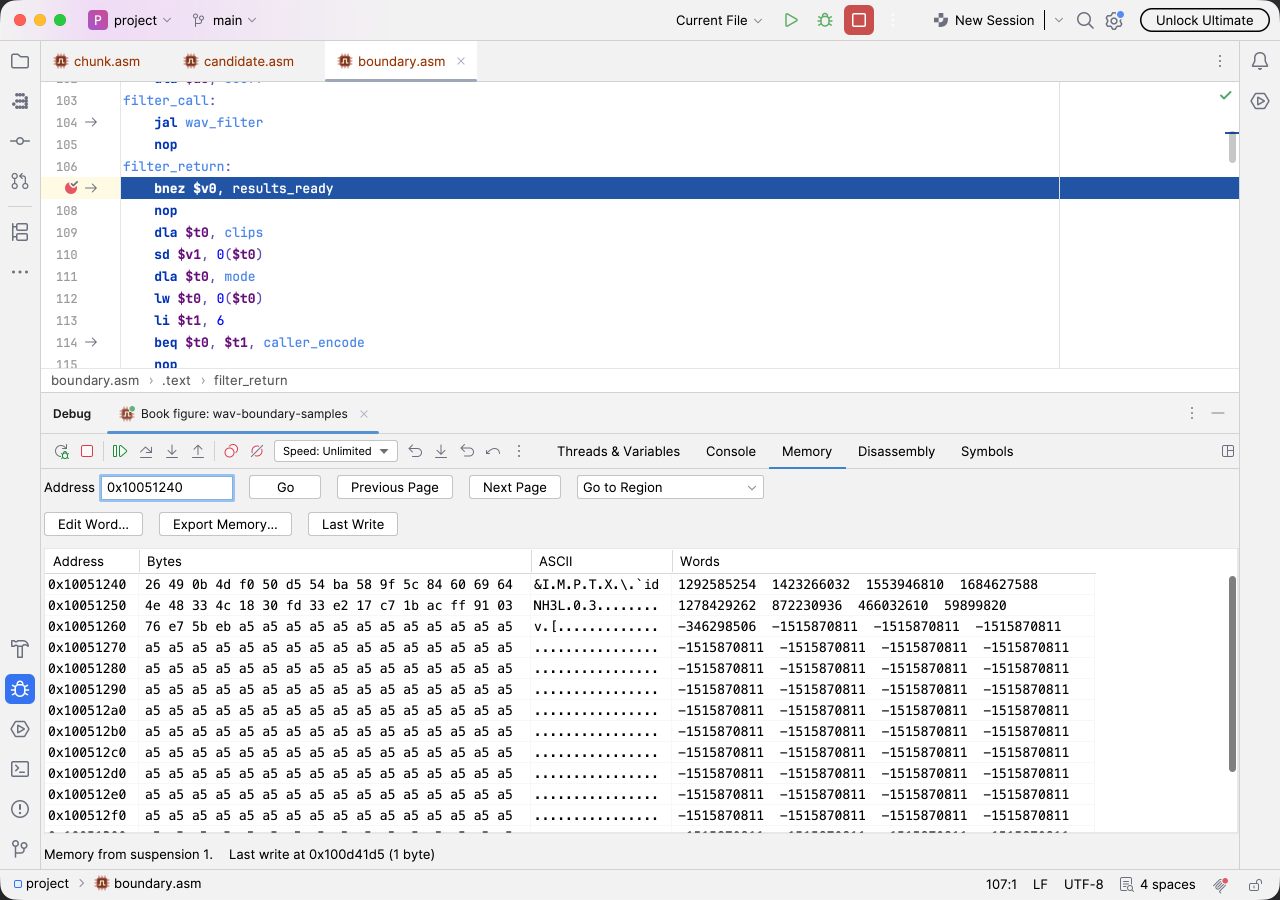
\includegraphics[width=0.84\linewidth,artifact,trim={\MARSwavboundaryoutputLeft{} \MARSwavboundaryoutputBottom{} \MARSwavboundaryoutputRight{} \MARSwavboundaryoutputTop{}},clip]{packages/031-pcm-wav/captures/f04/samples.png}};
\begin{scope}[shift={(output.south west)},x={($(output.south east)-(output.south west)$)},y={($(output.north west)-(output.south west)$)}]
\draw[black,line width=0.7pt] (0.194672131,0.043010753) rectangle (0.997950820,0.720430108);
\node[draw=black,fill=white,circle,inner sep=1.5pt,font=\footnotesize] at ($(0,0.720430108)+(-3mm,0)$) {3};
\end{scope}
\end{tikzpicture}
\par\smallskip
\begin{minipage}{\linewidth}
\small
\begin{enumerate}
\setlength{\itemsep}{0pt}
\setlength{\parsep}{0pt}
\item At \texttt{filter\_return}, both channels and both blocks have finished. The routine has restored its frame; the highlighted caller instruction has not yet tested the returned status.
\item \texttt{v0 = 0} reports success and \texttt{v1 = 0} reports clipped samples. This return value counts clips, not frames or output bytes. The input has 65 frames, split into blocks of 64 and one for each channel.
\item The rows show stereo frames 56 through 64, four bytes per frame. Frame 64 occupies the first four bytes of the final row; later \texttt{a5} bytes remain untouched. Independent integer checks compare every output sample and confirm that the final block begins with the previous seven input samples followed by its one new sample. History continues within a channel and resets only for the next channel.
\end{enumerate}
\end{minipage}
\caption{The sixty-five-frame result continues across the sixty-four-frame block boundary.}
\label{capture:031-pcm-wav-f04}
\label{pcm-wav-f04}
\end{figure}
\par
